\documentclass[tikz,border=8pt]{standalone}
\usepackage{amsmath,amssymb}
\usetikzlibrary{arrows.meta,calc,positioning}
\definecolor{ink}{HTML}{21352F}
\definecolor{teal}{HTML}{087F7B}
\definecolor{gold}{HTML}{C58B2A}
\definecolor{blue}{HTML}{4B77A8}
\definecolor{rose}{HTML}{B65A62}
\begin{document}
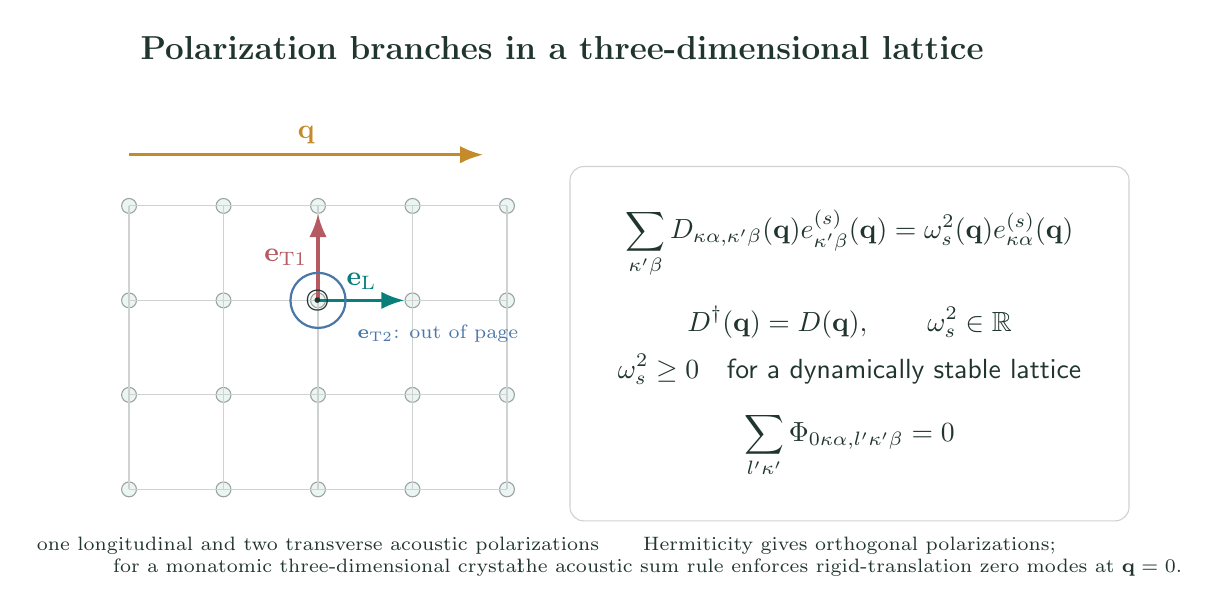
\begin{tikzpicture}[font=\sffamily,text=ink,>=Latex]
  \node[font=\bfseries\large] at (0,4.1) {Polarization branches in a three-dimensional lattice};
  \foreach \x in {-5.5,-4.3,-3.1,-1.9,-.7}{
    \foreach \y in {-1.5,-.3,.9,2.1}{
      \node[draw=ink!45,fill=teal!8,circle,inner sep=1.9pt] at (\x,\y) {};
    }
  }
  \foreach \x in {-5.5,-4.3,-3.1,-1.9}{
    \foreach \y in {-1.5,-.3,.9,2.1}{\draw[ink!22] (\x,\y)--++(1.2,0);}
  }
  \foreach \x in {-5.5,-4.3,-3.1,-1.9,-.7}{
    \foreach \y in {-1.5,-.3,.9}{\draw[ink!22] (\x,\y)--++(0,1.2);}
  }
  \draw[->,gold,very thick] (-5.5,2.75)--(-1.0,2.75) node[midway,above] {$\mathbf q$};
  \draw[->,teal,very thick] (-3.1,.9)--(-2.0,.9) node[midway,above] {$\mathbf e_{\rm L}$};
  \draw[->,rose,very thick] (-3.1,.9)--(-3.1,2.0) node[midway,left] {$\mathbf e_{\rm T1}$};
  \node[draw=blue,thick,circle,minimum size=7mm,inner sep=0pt] at (-3.1,.9) {$\boldsymbol\odot$};
  \node[blue,font=\scriptsize,anchor=west] at (-2.72,.48) {$\mathbf e_{\rm T2}$: out of page};
  \node[font=\scriptsize,align=center] at (-3.1,-2.35)
    {one longitudinal and two transverse acoustic polarizations\\for a monatomic three-dimensional crystal};

  \node[draw=ink!22,rounded corners=5pt,fill=white,minimum width=7.1cm,minimum height=4.5cm,align=center] at (3.65,.35) {
    $\displaystyle \sum_{\kappa'\beta}D_{\kappa\alpha,\kappa'\beta}(\mathbf q)
       e_{\kappa'\beta}^{(s)}(\mathbf q)
       =\omega_s^2(\mathbf q)e_{\kappa\alpha}^{(s)}(\mathbf q)$\\[9pt]
    $\displaystyle D^\dagger(\mathbf q)=D(\mathbf q),\qquad \omega_s^2\in\mathbb R$\\[5pt]
    $\displaystyle \omega_s^2\ge0\quad\text{for a dynamically stable lattice}$\\[9pt]
    $\displaystyle \sum_{l'\kappa'}\Phi_{0\kappa\alpha,l'\kappa'\beta}=0$
  };
  \node[font=\scriptsize,align=center] at (3.65,-2.35)
    {Hermiticity gives orthogonal polarizations;\\the acoustic sum rule enforces rigid-translation zero modes at $\mathbf q=0$.};
\end{tikzpicture}
\end{document}
